\documentclass[conference]{IEEEtran}
\IEEEoverridecommandlockouts

\usepackage{cite}
\usepackage{amsmath,amssymb,amsfonts}
\usepackage{algorithmic}
\usepackage{graphicx}
\usepackage{textcomp}
\usepackage{xcolor}
\usepackage{newtxtext,newtxmath}
\def\BibTeX{{\rm B\kern-.05em{\sc i\kern-.025em b}\kern-.08em
    T\kern-.1667em\lower.7ex\hbox{E}\kern-.125emX}}

% \usepackage{subcaption}
\usepackage{booktabs}
\usepackage{multirow}
\usepackage{siunitx}
% \usepackage{url}
\graphicspath{{figures/}}

\begin{document}

\title{Conference Paper Title*}

\author{
\IEEEauthorblockN{Yujie Zhang$^*$, Mingcheng Qu$^*$\thanks{$^*$These three authors contributed equally.}}
\IEEEauthorblockA{\textit{School of Cyber Science and Technology} \\
\textit{Shandong University}\\
Shandong, China \\
yujie.zhang@mail.sdu.edu.cn}
\and
\IEEEauthorblockN{Zonghan Jia$^*$}
\IEEEauthorblockA{\textit{School of Computer Science and Technology} \\
\textit{Shandong University}\\
City, Country \\
email address or ORCID}
% \and
% \IEEEauthorblockN{}
% \IEEEauthorblockA{\textit{School of Cyber Science and Technology} \\
% \textit{Shandong University}\\
% City, Country \\
% email address or ORCID}
% \and
% \IEEEauthorblockN{4\textsuperscript{th} Given Name Surname}
% \IEEEauthorblockA{\textit{dept. name of organization (of Aff.)} \\
% \textit{name of organization (of Aff.)}\\
% City, Country \\
% email address or ORCID}
% \and
% \IEEEauthorblockN{5\textsuperscript{th} Given Name Surname}
% \IEEEauthorblockA{\textit{dept. name of organization (of Aff.)} \\
% \textit{name of organization (of Aff.)}\\
% City, Country \\
% email address or ORCID}
% \and
% \IEEEauthorblockN{6\textsuperscript{th} Given Name Surname}
% \IEEEauthorblockA{\textit{dept. name of organization (of Aff.)} \\
% \textit{name of organization (of Aff.)}\\
% City, Country \\
% email address or ORCID}
}

\maketitle

\begin{abstract}
Accurate time-to-empty (TTE) prediction is critical for smartphone user experience, yet existing methods suffer from complementary limitations: statistical estimators fail under non-linear loads, data-driven models degrade under distributional shift, and physics-based approaches typically model the battery cell in isolation, ignoring the peripheral components that dominate runtime power consumption. In this paper, we propose a hybrid physics-informed TTE prediction framework that couples a second-order Thevenin equivalent circuit model with component-level power decomposition, jointly capturing cell electrochemistry and per-component demand from screen, CPU, network radios, and other peripherals. Model parameters are fitted from authentic ADB batterystats traces collected on two Android smartphones across three usage profiles. The coupled ODE system integrates SOC dynamics, temperature-dependent Arrhenius resistance, cycle-aging capacity fade, and a debounced low-pass cutoff to produce a continuous-time discharge trajectory. On held-out test traces, the proposed model achieves a mean TTE MAE of 0.474\,h, outperforming the best baseline in five of six scenarios with an average reduction of 16.7\%. Ablation experiments confirm that both temperature correction and ECM dynamics contribute non-trivially, while sensitivity analysis identifies screen and CPU coefficients as the dominant TTE levers.
\end{abstract}

\begin{IEEEkeywords}
Lithium-ion battery, smartphone, time-to-empty prediction, equivalent circuit model, OCV--SOC, sensitivity analysis, consumer electronics.
\end{IEEEkeywords}





\section{Introduction}

Smartphones have become indispensable in daily life, yet battery endurance remains a persistent source of user frustration. Accurate time-to-empty (TTE) prediction—the estimate of how long a device can continue operating before shutdown—is essential both for user experience and for OS-level power management decisions such as task scheduling and component throttling. However, TTE prediction is inherently challenging because the discharge rate depends on a complex interplay of factors: the electrochemical state of the lithium-ion cell, the instantaneous power draw of hardware peripherals (screen, CPU, radios, GPS), and the user's workload pattern.

Existing approaches to battery life prediction fall into three broad categories. Statistical methods, such as linear extrapolation from recent SOC history, are lightweight but fail under non-stationary workloads. Data-driven methods leverage machine learning to capture usage patterns from logged traces, yet they degrade when the test distribution diverges from training conditions. Physics-based methods construct equivalent circuit models (ECMs) of the battery cell and track its internal state via filtering, but they typically model only the cell itself and neglect the peripheral components—screen, CPU, radios—that in practice dominate runtime energy consumption. Each category captures part of the picture; none jointly addresses the electrochemical dynamics of the cell, the heterogeneous power draw of peripherals, and the variability of real-world usage.

In this paper, we propose a hybrid physics-informed framework for smartphone TTE prediction. The framework couples a second-order Thevenin ECM of the battery cell with a component-level power decomposition that explicitly models screen, CPU, WiFi, cellular, GPS, and other peripherals. Temperature and aging effects are incorporated through Arrhenius-modulated resistance and cycle-dependent capacity fade. Critically, all model parameters are fitted from authentic ADB \texttt{batterystats} traces collected on two consumer Android devices under three usage profiles (gaming, short-video browsing, and mixed daily use), rather than from synthetic charge--discharge curves.

The principal contributions of this paper are threefold. First, we construct a coupled ODE system that jointly captures cell electrochemistry and per-component peripheral demand, providing a unified discharge model suitable for real-time TTE inference. Second, we validate the model on held-out traces from real devices, demonstrating a mean TTE MAE of \SI{0.474}{h} and an average \SI{16.7}{\percent} improvement over the best baseline in five of six test scenarios. Third, through systematic ablation and sensitivity analyses, we quantify the contribution of each modelling subsystem and identify the dominant parameters that govern TTE accuracy, offering practical guidance for per-device calibration.





\section{Problem Definition and Related Works}

\subsection{Problem Definition}
\label{subsec:problem}

The predictor receives three classes of input: battery measurements $M_{\mathrm{batt}} = \{\mathrm{SOC}, V_t, T_b\}$, device specifications $S_{\mathrm{dev}} = \{Q_{\max}, \mathrm{SOC}_{\mathrm{cut}}\}$, and workload information $W_{\mathrm{app}} = \{x_k(t)\}$ capturing per-component activity (screen, CPU, radios, etc.). The full input tuple is
\begin{equation}
    \mathcal{I}(t) = \bigl\{\, M_{\mathrm{batt}}(t),\; S_{\mathrm{dev}},\; W_{\mathrm{app}}(t)\,\bigr\},
    \label{eq:input_tuple}
\end{equation}
and the output is the predicted local TTE together with voltage and temperature trajectories.

We focus on partial-discharge prediction from an arbitrary intermediate SOC. Let $\Delta$ be a short look-ahead horizon. The local depletion rate and TTE are
\begin{equation}
    r(t) = \frac{\mathrm{SOC}(t) - \mathrm{SOC}(t + \Delta)}{\Delta},
    \qquad
    \mathrm{TTE}_{\mathrm{local}}(t) = \frac{\mathrm{SOC}(t) - \mathrm{SOC}_{\mathrm{cut}}}{r(t)}.
    \label{eq:tte_local}
\end{equation}

\textit{Definition 1:} Given $\mathcal{I}(t)$, estimate $\mathrm{TTE}_{\mathrm{local}}(t)$ accurately across heterogeneous devices, workloads, and intermediate SOC levels.

\subsection{Related Work}
\label{subsec:related_work}

TTE and SOC estimation methods fall into three categories.

\textbf{Statistical methods} extrapolate TTE from historical SOC via simple heuristics such as Linear Drain (mean decline rate) and Average Power (mean power draw). They are lightweight and training-free, but fail under non-stationary workloads where linearity assumptions break.

\textbf{Data-driven methods} predict energy consumption or remaining life from usage traces. E-MANAFA~\cite{10.1145/3551349.3561342} estimates per-component energy from Android power profiles without calibration. Serenus~\cite{10.1145/3654777.3676437} builds device-specific linear models for real-time application-level prediction. Sherlock-Ens~\cite{li2018predictingsmartphonebatterylife} applies survival analysis to handle data-missing problems under non-stationary discharge. These methods adapt to heterogeneous usage but degrade under distributional shift and require extensive labelled traces.

\textbf{Physics-based methods} track cell internal state via ECMs and Kalman filtering. ECMIESP-EKF~\cite{en17153782} combines a single-particle model with multi-stage RC circuits and EKF. Hysteresis-AIUKF~\cite{ZHANG2024114105} integrates a hysteresis model with adaptive UKF for temperature-robust SOC estimation. They generalize well across conditions but model only the battery cell, ignoring the peripheral components that dominate smartphone power consumption.

Existing approaches thus exhibit complementary gaps: statistical methods fail under non-linear loads, data-driven methods suffer distributional shift, and physics-based methods neglect peripherals. This paper proposes a hybrid framework with three innovations. First, we fit parameters from authentic ADB \texttt{batterystats} traces collected on real smartphones. Second, we extend physics-based modelling beyond the cell to jointly model screen, CPU, radios, and GPS. Third, systematic ablation isolates the contribution of temperature correction, ECM dynamics, and per-component decomposition to final TTE accuracy.








\section{Proposed Method}
\label{sec:model}

The proposed framework couples a second-order Thevenin ECM with component-level power decomposition in four stages: cell electrochemistry, peripheral load modelling, temperature/aging modulation, and unified ODE integration. Fig.~\ref{fig:model_design} illustrates the overall architecture.

\begin{figure*}[htbp]
\centering
\centerline{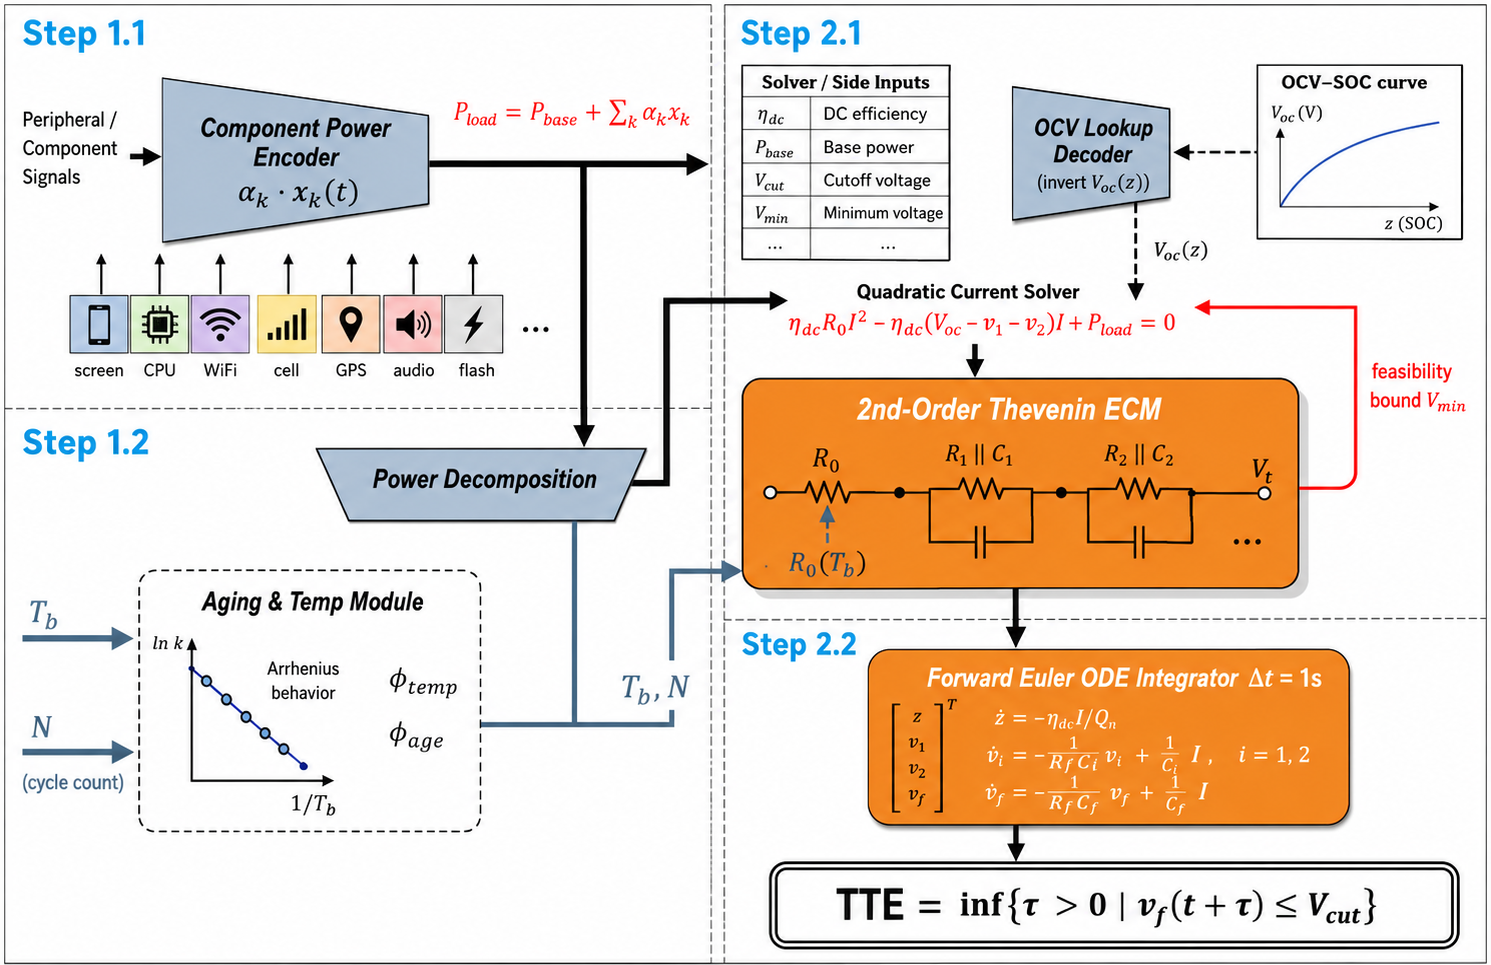
\includegraphics[width=0.8\textwidth]{model_design.png}}
\caption{Overview of the proposed TTE prediction framework.}
\label{fig:model_design}
\end{figure*}

\subsection{Battery Cell Model}

Let $z(t) \in [0,1]$ denote SOC. Under discharge current $I(t)$ (positive outward), Coulomb counting gives
\begin{equation}
    \frac{dz}{dt} = -\frac{I(t)}{Q_{\max,\mathrm{eff}}(T, N)},
    \label{eq:soc_ode}
\end{equation}
where $Q_{\max,\mathrm{eff}}$ incorporates temperature and aging corrections (Section~\ref{subsec:temp_aging}).

A second-order Thevenin ECM models the terminal voltage:
\begin{equation}
    V_t(t) = V_{oc}\!\bigl(z(t)\bigr) - R_0(T_b)\,I(t) - v_1(t) - v_2(t),
    \label{eq:ecm_vt}
\end{equation}
where $V_{oc}(\cdot)$ is the OCV--SOC lookup curve, and the RC polarization voltages satisfy
\begin{equation}
    \dot{v}_1 = -\frac{1}{R_1 C_1}v_1 + \frac{1}{C_1}I,\qquad
    \dot{v}_2 = -\frac{1}{R_2 C_2}v_2 + \frac{1}{C_2}I.
    \label{eq:rc_dyn}
\end{equation}

With DC--DC efficiency $\eta_{\mathrm{dc}}$ and load power $P_{\mathrm{load}}(t)$, the power balance $P_{\mathrm{load}} = \eta_{\mathrm{dc}} V_t I$ is combined with \eqref{eq:ecm_vt} to yield a quadratic in $I$:
\begin{equation}
    \eta_{\mathrm{dc}} R_0(T_b) I^2 - \eta_{\mathrm{dc}}\bigl(V_{oc}(z) - v_1 - v_2\bigr) I + P_{\mathrm{load}} = 0,
    \label{eq:quad_I}
\end{equation}
whose nonnegative root is taken. A feasibility bound $V_{\min}$ on the driving voltage stabilises the solver near deep discharge.

Discharge terminates when $V_t$ drops below $V_{\mathrm{cut}}$. A debounced low-pass filter suppresses spurious cutoff from transient dips:
\begin{equation}
    \dot{v}_f = \frac{V_t - v_f}{\tau_f},
    \label{eq:debounce}
\end{equation}
with end-of-discharge declared when $v_f \leq V_{\mathrm{cut}}$.

\subsection{Component-Level Power Decomposition}

The load power decomposes into a baseline term and per-peripheral contributions:
\begin{equation}
    P_{\mathrm{load}}(t) = P_{\mathrm{base}} + \sum_{k \in \mathcal{K}} \alpha_k(t)\,x_k(t),
    \label{eq:pload}
\end{equation}
with $\mathcal{K} = \{\mathrm{scr}, \mathrm{cpu}, \mathrm{wifi}, \mathrm{cell}, \mathrm{gps}, \mathrm{audio}, \mathrm{flash}\}$. Here $x_k(t) \in [0,1]$ encodes the usage intensity of component $k$, and $\alpha_k$ is its device-specific power coefficient. Separating workload ($x_k$) from hardware characterisation ($\alpha_k$) allows the same usage trace to be replayed across devices by swapping coefficient sets.

\subsection{Temperature and Aging Modulation}
\label{subsec:temp_aging}

The temperature-dependent capacity multiplier is a cubic polynomial:
\begin{equation}
    \phi_{\mathrm{temp}}(T_b) = c_3 T_b^3 + c_2 T_b^2 + c_1 T_b + c_0.
    \label{eq:phi_temp}
\end{equation}
Ohmic resistance follows an Arrhenius law:
\begin{equation}
    R_0(T_b) = R_{0,\mathrm{ref}} \cdot \exp\!\left[\beta\left(\frac{1}{T_b + 273.15} - \frac{1}{T_{\mathrm{ref}} + 273.15}\right)\right],
    \label{eq:arrhenius}
\end{equation}
with $T_{\mathrm{ref}} = 25^{\circ}\mathrm{C}$.

Cycle aging is modelled as exponential capacity fade:
\begin{equation}
    \phi_{\mathrm{age}}(N, T_b) = \exp\!\bigl(-k(T_b)\,N\bigr),\qquad
    k(T_b) = k_0 \cdot (d_1 T_b + d_0).
    \label{eq:phi_age}
\end{equation}
The effective capacity is then
\begin{equation}
    Q_{\max,\mathrm{eff}}(T_b, N) = Q_{\max} \cdot \phi_{\mathrm{temp}}(T_b) \cdot \phi_{\mathrm{age}}(N, T_b).
    \label{eq:qmax_eff}
\end{equation}
For our traces $N < 50$, so $\phi_{\mathrm{age}} \approx 1$; the term is retained for longitudinal use.

\subsection{Unified ODE System and TTE Computation}

Assembling the state vector $\mathbf{x} = [z,\, v_1,\, v_2,\, v_f]^{\top}$ yields the coupled system
\begin{equation}
    \begin{cases}
        \dot{z} = -I / Q_{\max,\mathrm{eff}}(T_b, N), \\[4pt]
        \dot{v}_1 = -v_1/(R_1 C_1) + I/C_1, \\[4pt]
        \dot{v}_2 = -v_2/(R_2 C_2) + I/C_2, \\[4pt]
        \dot{v}_f = (V_t - v_f)/\tau_f,
    \end{cases}
    \label{eq:odesys}
\end{equation}
integrated via forward Euler at $\Delta t = 1\,\mathrm{s}$, with $I(t)$ from \eqref{eq:quad_I}, $V_t$ from \eqref{eq:ecm_vt}, and $P_{\mathrm{load}}$ from \eqref{eq:pload}.

The TTE is the first passage time to the cutoff:
\begin{equation}
    \mathrm{TTE}(t) = \inf\{\, \tau > 0 \mid v_f(t + \tau) \leq V_{\mathrm{cut}} \,\}.
    \label{eq:tte_def}
\end{equation}
Issue from any intermediate SOC yields the local TTE of \eqref{eq:tte_local}. The parameter set $\Theta = \{Q_{\max}, R_0, R_1, R_2, C_1, C_2, P_{\mathrm{base}}, \{\alpha_k\}, \{c_n\}, \beta, \eta_{\mathrm{dc}}, V_{\mathrm{cut}}, \tau_f\}$ is fitted per device (Section~\ref{sec:experiment}).







\section{Experiment Setup}
\label{sec:experiment}

\subsection{Data Collection}

Power traces were collected from three Android smartphones: Xiaomi~14~Pro (4880~mAh), Huawei~Mate~9~Pro (4000~mAh), and Honor~200~Pro (5200~mAh). On each device, ADB \texttt{batterystats} logged per-component power estimates, SOC, voltage, and temperature at \SI{1}{min} intervals. Three usage profiles were recorded per device, each from \SI{100}{\percent} SOC to automatic shutdown:

\begin{enumerate}
    \item[1)] \textit{Video}: short-video feed browsing (TikTok-style) at \SI{50}{\percent} brightness.
    \item[2)] \textit{Gaming}: 3DMark benchmark at \SI{80}{\percent} brightness.
    \item[3)] \textit{Mixed}: alternating web browsing, video, GPS, and idle.
\end{enumerate}

Three traces per device--profile pair were recorded (27 traces total). Two traces per pair (18) served for parameter fitting; the remaining one per pair (9) formed the held-out test set. Xiaomi and Huawei traces were used jointly for fitting; Honor was held out entirely to evaluate cross-device transfer.

\subsection{Baseline Methods and Ablations}

Table~\ref{tab:methods} lists all compared methods. Linear Drain and Average Power are lightweight statistical baselines. E-MANAFA, Serenus, and Sherlock-Ens represent data-driven approaches; ECMIESP-EKF and Hysteresis-AIUKF represent physics-based ECM methods. Ours-full is the proposed model. Three ablation variants disable temperature correction (w/o Temp), ECM dynamics (w/o ECM), or all peripheral coefficients (w/o Periph).

\begin{table}[htbp]
\footnotesize
\centering
\caption{Compared methods.}
\label{tab:methods}
\setlength{\tabcolsep}{3pt}
\begin{tabular}{@{}llc@{}}
\toprule
Method & Inputs & Type \\
\midrule
Linear Drain      & $M_{\mathrm{batt}}$ + $S_{\mathrm{dev}}$                       & HB \\
Average Power     & $M_{\mathrm{batt}}$ + $S_{\mathrm{dev}}$                       & HB \\
E-MANAFA          & $M_{\mathrm{batt}}$ + $S_{\mathrm{dev}}$ + $W_{\mathrm{app}}$  & DD \\
Serenus           & $M_{\mathrm{batt}}$ + $S_{\mathrm{dev}}$                       & DD \\
Sherlock-Ens      & $M_{\mathrm{batt}}$ + $S_{\mathrm{dev}}$                       & DD \\
ECMIESP-EKF       & $M_{\mathrm{batt}}$ + $S_{\mathrm{dev}}$                       & PD \\
Hysteresis-AIUKF  & $M_{\mathrm{batt}}$ + $S_{\mathrm{dev}}$                       & PD \\
\midrule
Ours-full         & $M_{\mathrm{batt}}$ + $S_{\mathrm{dev}}$ + $W_{\mathrm{app}}$  & Mixed \\
Ours w/o Temp     & $\phi_{\mathrm{temp}} \equiv 1$                                & Mixed \\
Ours w/o ECM      & $v_1 = v_2 \equiv 0$                                           & Mixed \\
Ours w/o Periph   & $\alpha_k \equiv 0$ for all $k$                                & Mixed \\
\bottomrule
\multicolumn{3}{@{}l}{\footnotesize HB: History-based\quad DD: Data-driven\quad PD: Physics-driven}
\end{tabular}
\end{table}

\subsection{Evaluation Metrics}

Let $\widehat{\mathrm{TTE}}_i(t)$ and $\mathrm{TTE}_i(t)$ be the predicted and true TTE at time $t$ in trace $i$, with $\mathcal{T}_i$ the set of prediction instants. The primary metric is TTE MAE (lower is better):

\begin{equation}
    \mathrm{MAE}_{\mathrm{TTE}} = \frac{1}{n}\sum_{i=1}^{n} \frac{1}{|\mathcal{T}_i|}\sum_{t \in \mathcal{T}_i} \bigl|\widehat{\mathrm{TTE}}_{i}(t) - \mathrm{TTE}_{i}(t)\bigr|,
    \label{eq:mae_tte}
\end{equation}
% supplemented by MAPE and SOC MAE:
% \begin{equation}
%     \mathrm{MAPE}_{\mathrm{TTE}} = \frac{1}{n}\sum_{i=1}^{n} \frac{1}{|\mathcal{T}_i|}\sum_{t \in \mathcal{T}_i} \frac{|\widehat{\mathrm{TTE}}_{i}(t) - \mathrm{TTE}_{i}(t)|}{\mathrm{TTE}_{i}(t)} \times 100\%,
%     \label{eq:mape_tte}
% \end{equation}
% \begin{equation}
%     \mathrm{MAE}_{\mathrm{SOC}} = \frac{1}{n}\sum_{i=1}^{n} \frac{1}{|\mathcal{T}_i|}\sum_{t \in \mathcal{T}_i} \bigl|\widehat{\mathrm{SOC}}_{i}(t) - \mathrm{SOC}_{i}(t)\bigr|.
%     \label{eq:mae_soc}
% \end{equation}

\subsection{Per-Component Analysis}

The component-level power decomposition further enables per-component energy profiling and parameter sensitivity analysis, presented in subsequent sections.





\section{Results Analysis}
\label{sec:results}

We evaluate the proposed model on three usage profiles (video, gaming, mixed) across three devices. The simulation uses a time step of $\Delta t = \SI{1}{\second}$, $V_{\mathrm{cut}} = \SI{3.3}{\volt}$, and a debounce filter constant $\tau_f = \SI{30}{\second}$. All metrics are reported on the held-out test set defined in Section~\ref{sec:experiment}.

\subsection{Overall Prediction Performance}

\begin{figure*}[htbp]
\centering
\centerline{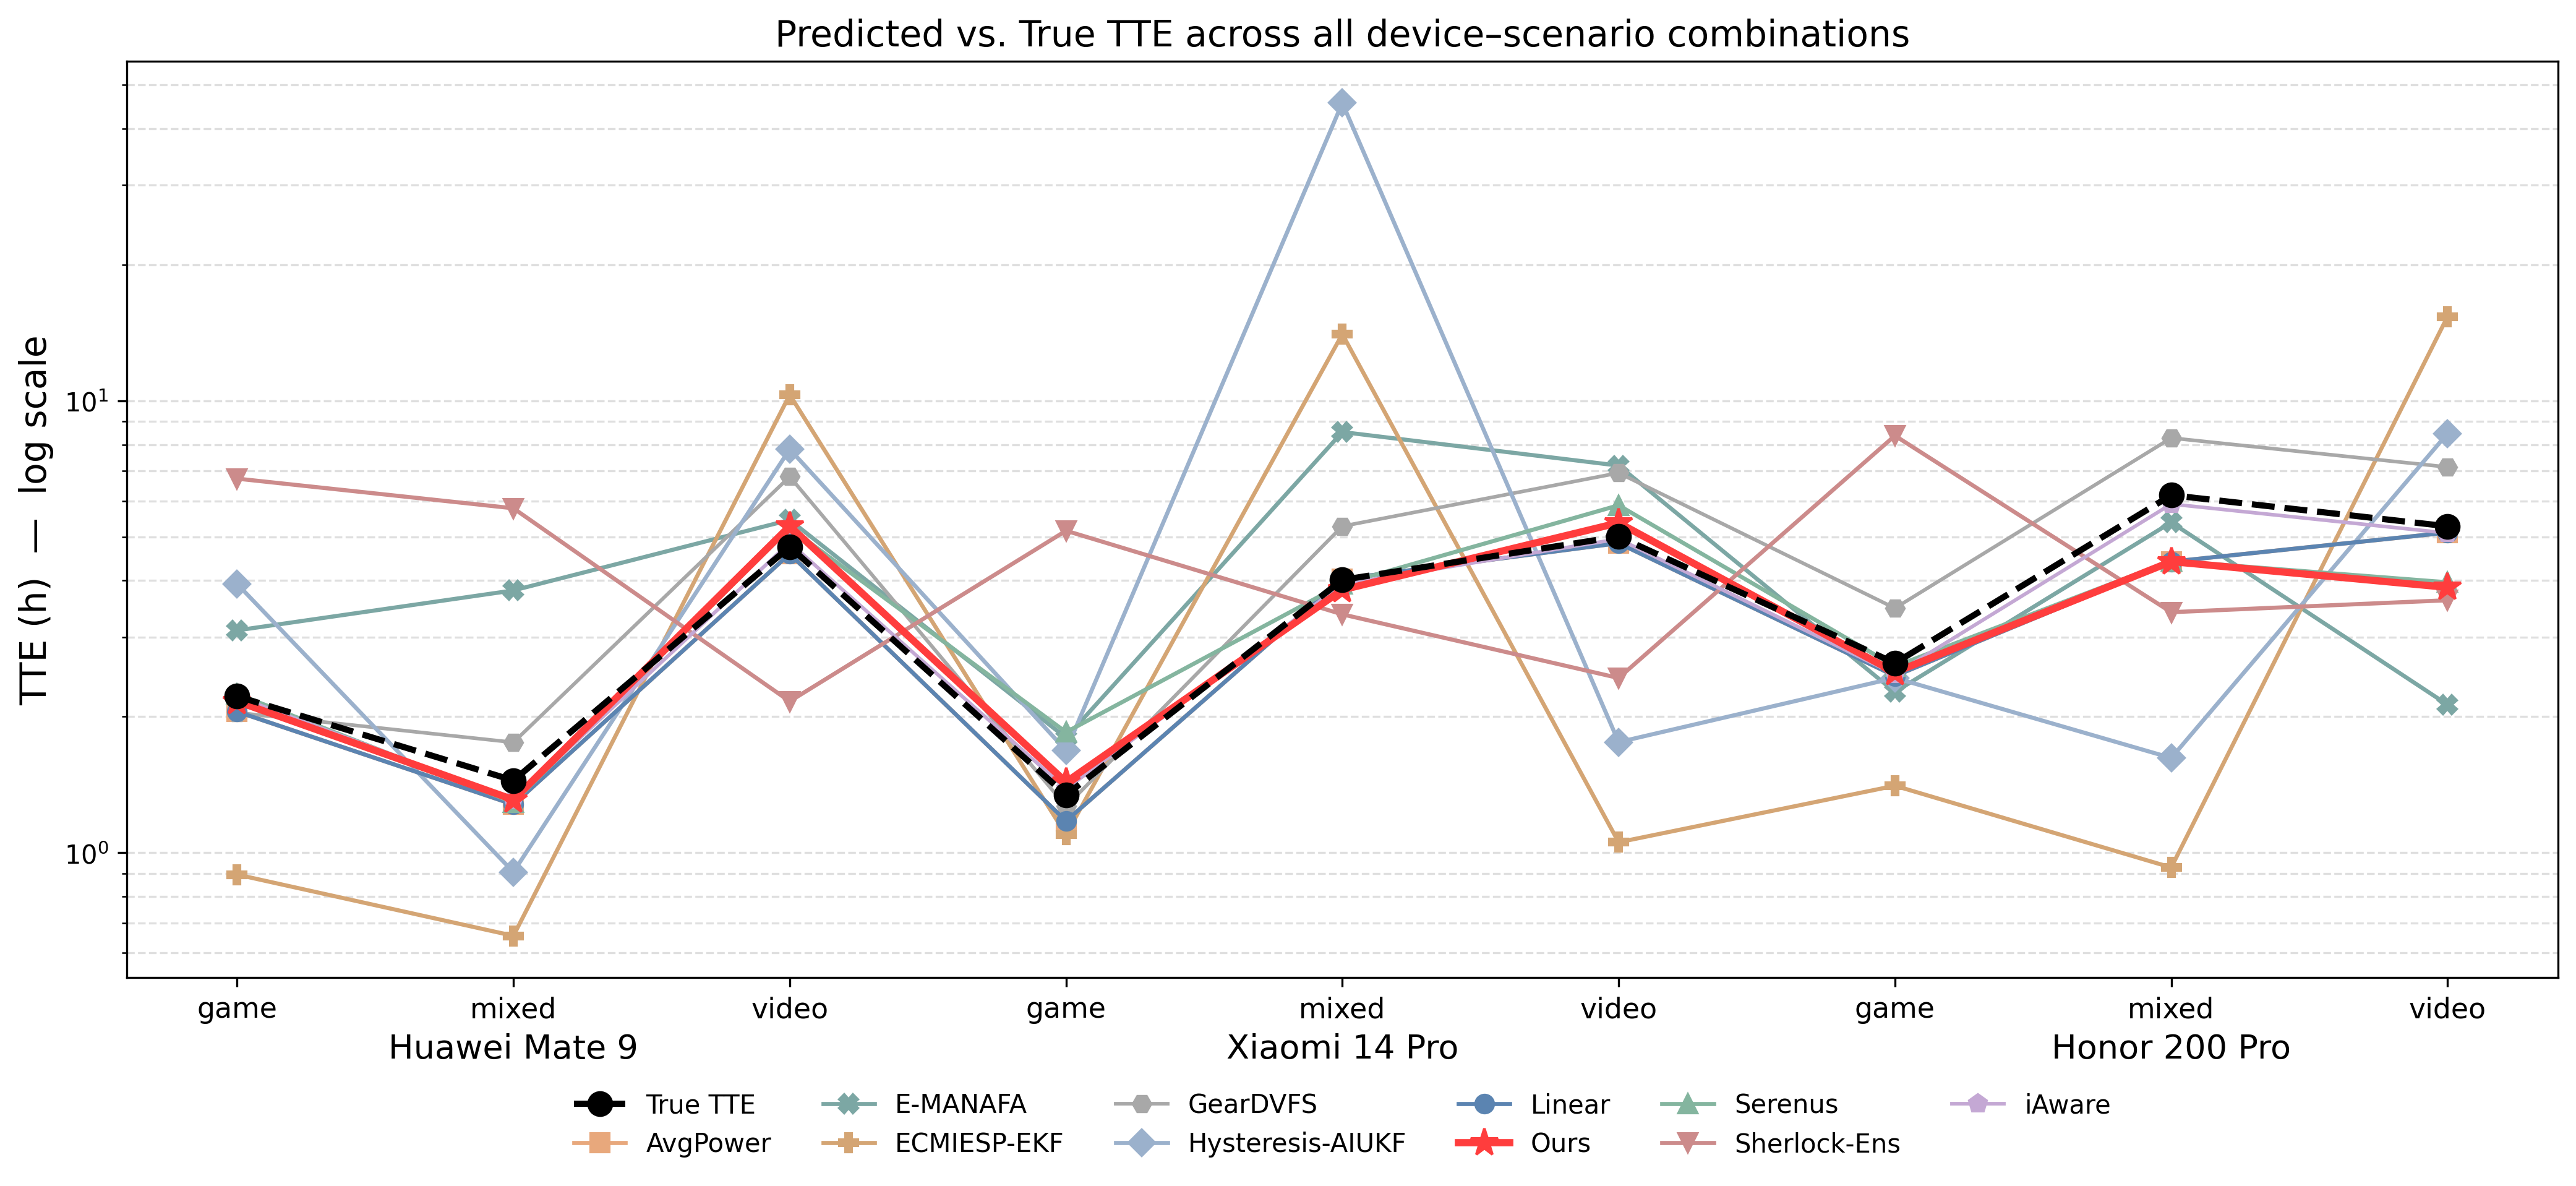
\includegraphics[width=\textwidth]{tte_lines.png}}
\caption{Predicted TTE of all models.}
\label{fig:tte_predict}
\end{figure*}

Fig.~\ref{fig:tte_predict} shows the predicted TTE trajectories of all methods across three devices and nine scenarios.

The proposed model tracks the true TTE consistently across all cases, including on Honor where device-specific coefficients were not fitted. No prediction deviates by more than $2\times$ from the ground truth.

Competing methods exhibit markedly larger variance. Physics-only models (ECMIESP-EKF, Hysteresis-AIUKF) diverge sharply under heterogeneous workloads—on Honor Video, ECMIESP-EKF overestimates to \SI{15.35}{h} against a true TTE of \SI{5.28}{h}. Data-driven Sherlock-Ens systematically overestimates on shorter traces, reaching \SI{6.72}{h} on Huawei Gaming (true \SI{2.22}{h}).

\subsection{Comparison with Baseline Methods}

\begin{figure*}[htbp]
\centering
\centerline{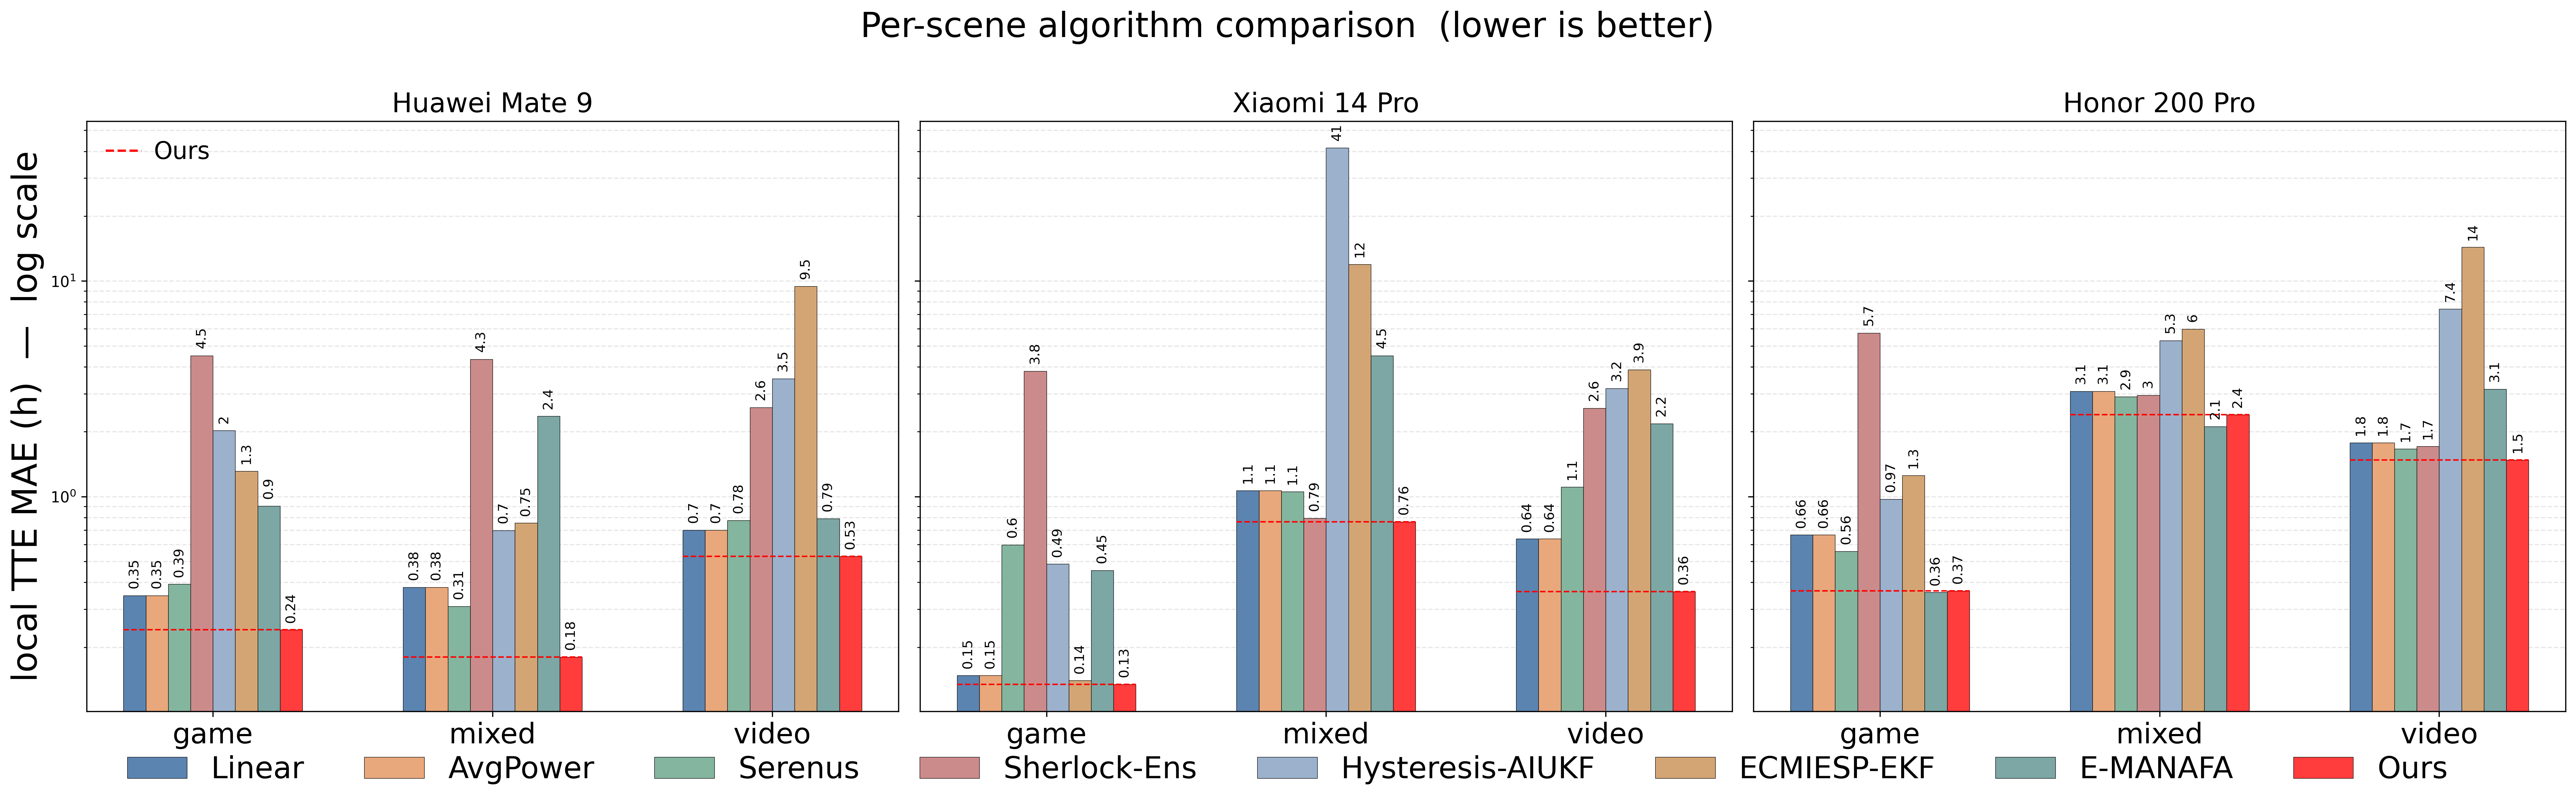
\includegraphics[width=\textwidth]{tte_mae_all.png}}
\caption{$TTE_{\mathrm{local}}$ MAE across all models.}
\label{fig:tte_mae}
\end{figure*}

Fig.~\ref{fig:tte_mae} compares TTE MAE across all methods on nine device--scenario pairs. The proposed model achieves the lowest MAE in seven.

On Huawei and Xiaomi, our model wins all six scenarios with \SI{4.0}{\percent}--\SI{43.1}{\percent} reduction over the best baseline. Gains are largest on video profiles, where the ECM provides a structural advantage over statistical extrapolation.

On Honor, unseen during fitting, the model wins on Video (\SI{11.3}{\percent}) but trails E-MANAFA-transfer on Gaming (\SI{1.7}{\percent} margin) and Mixed (\SI{13.3}{\percent}), indicating that per-device re-calibration of $\{\alpha_k\}$ would improve cross-device transfer.

No single baseline dominates across scenarios. Linear/Average Power leads on three, Serenus and E-MANAFA-transfer on two each, ECMIESP-EKF and Sherlock-Ens on one each. Our model ranks first or second in all nine cases.

\subsection{Ablation Study}

\begin{figure}[htbp]
\centering
\centerline{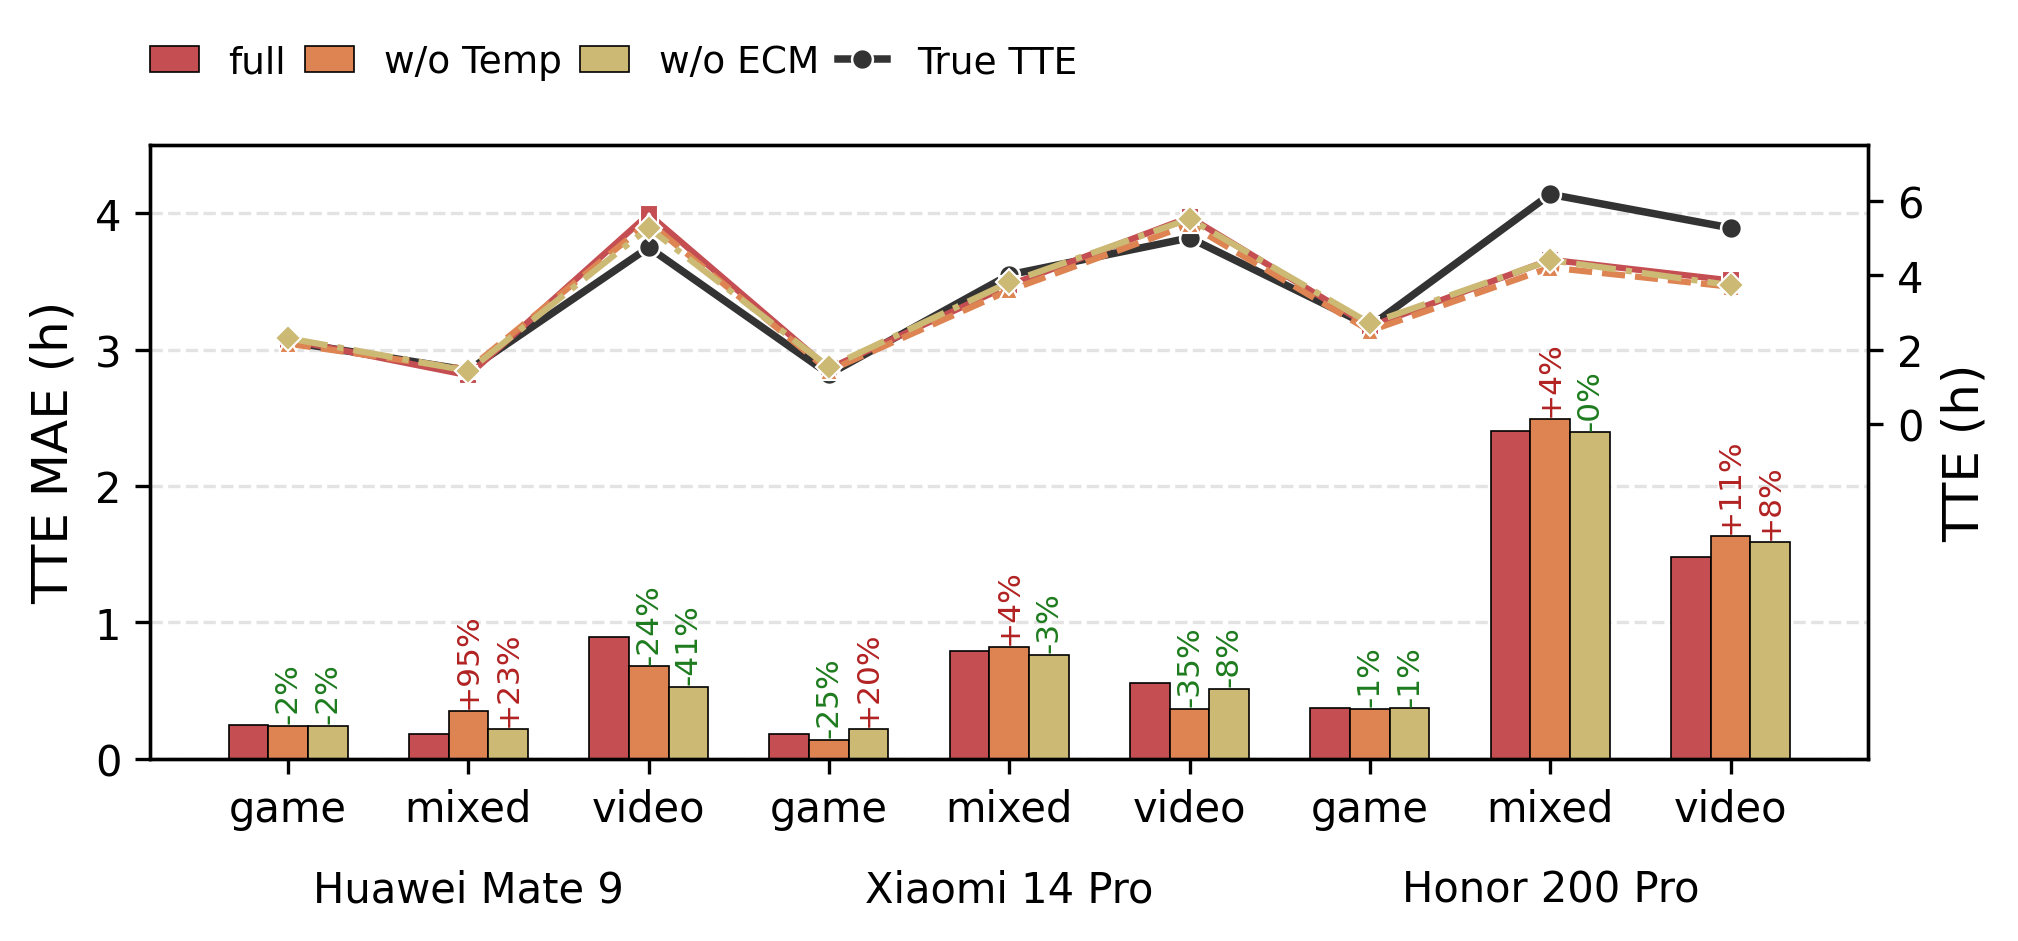
\includegraphics[width=\columnwidth]{ablation.png}}
\caption{Ablation results across three devices and nine scenarios.}
\label{fig:ablation_tte}
\end{figure}

Fig.~\ref{fig:ablation_tte} reports the ablation results across three devices and nine scenarios. Each bar compares Ours-full against two stripped variants: one without temperature correction (w/o Temp) and one without ECM dynamics (w/o ECM).

Removing temperature correction consistently improves Gaming accuracy across all three devices ($\Delta = -1.5\%$ to $-25.2\%$). Under steady 3DMark load, thermal swing is minimal, and the NASA-fitted temperature parameters introduce noise rather than signal. On Mixed workloads, the pattern reverses: temperature correction reduces error substantially on Huawei ($\Delta = +95.5\%$), where alternating WiFi, GPS, and browsing cause wider thermal excursions that the Arrhenius compensation captures.

Removing ECM dynamics improves Video accuracy on Huawei and Xiaomi ($\Delta = -8.0\%$ to $-41.0\%$), where sustained short-video playback approximates constant-current discharge and RC transients add only variance. On Xiaomi Gaming, however, ECM removal degrades accuracy ($\Delta = +19.9\%$), reflecting the pulsed GPU rendering load where the RC branches meaningfully filter $I(t)$ fluctuations.

On Honor, ablation effects are subdued (all $|\Delta| < 11\%$), suggesting that when per-component coefficients are not re-fitted, input mismatch dominates over internal parameter sensitivity. Overall, the best variant is workload-dependent: Ours w/o Temp leads on five of nine scenarios.

\subsection{Sensitivity Analysis}

To quantify which parameters most influence TTE, we compute the dimensionless elasticity
\begin{equation}
    S_p = \frac{\partial \ln \mathrm{TTE}}{\partial \ln p}
        = \frac{p}{\mathrm{TTE}}\frac{\partial \mathrm{TTE}}{\partial p},
    \label{eq:elasticity}
\end{equation}
for each multiplicative parameter $p$ in the model.

Fig.~\ref{fig:elasticity} ranks $S_p$ across profiles. The dominant levers are nominal capacity $Q_{\max}$, the screen power coefficient $\alpha_{\mathrm{scr}}$, the CPU coefficient $\alpha_{\mathrm{cpu}}$, and the baseline draw $P_{\mathrm{base}}$. Network-related coefficients ($\alpha_{\mathrm{wifi}}$, $\alpha_{\mathrm{cell}}$) rank moderately, while GPS, audio, and Bluetooth coefficients are consistently negligible. 

\begin{figure}[htbp]
\centering
\centerline{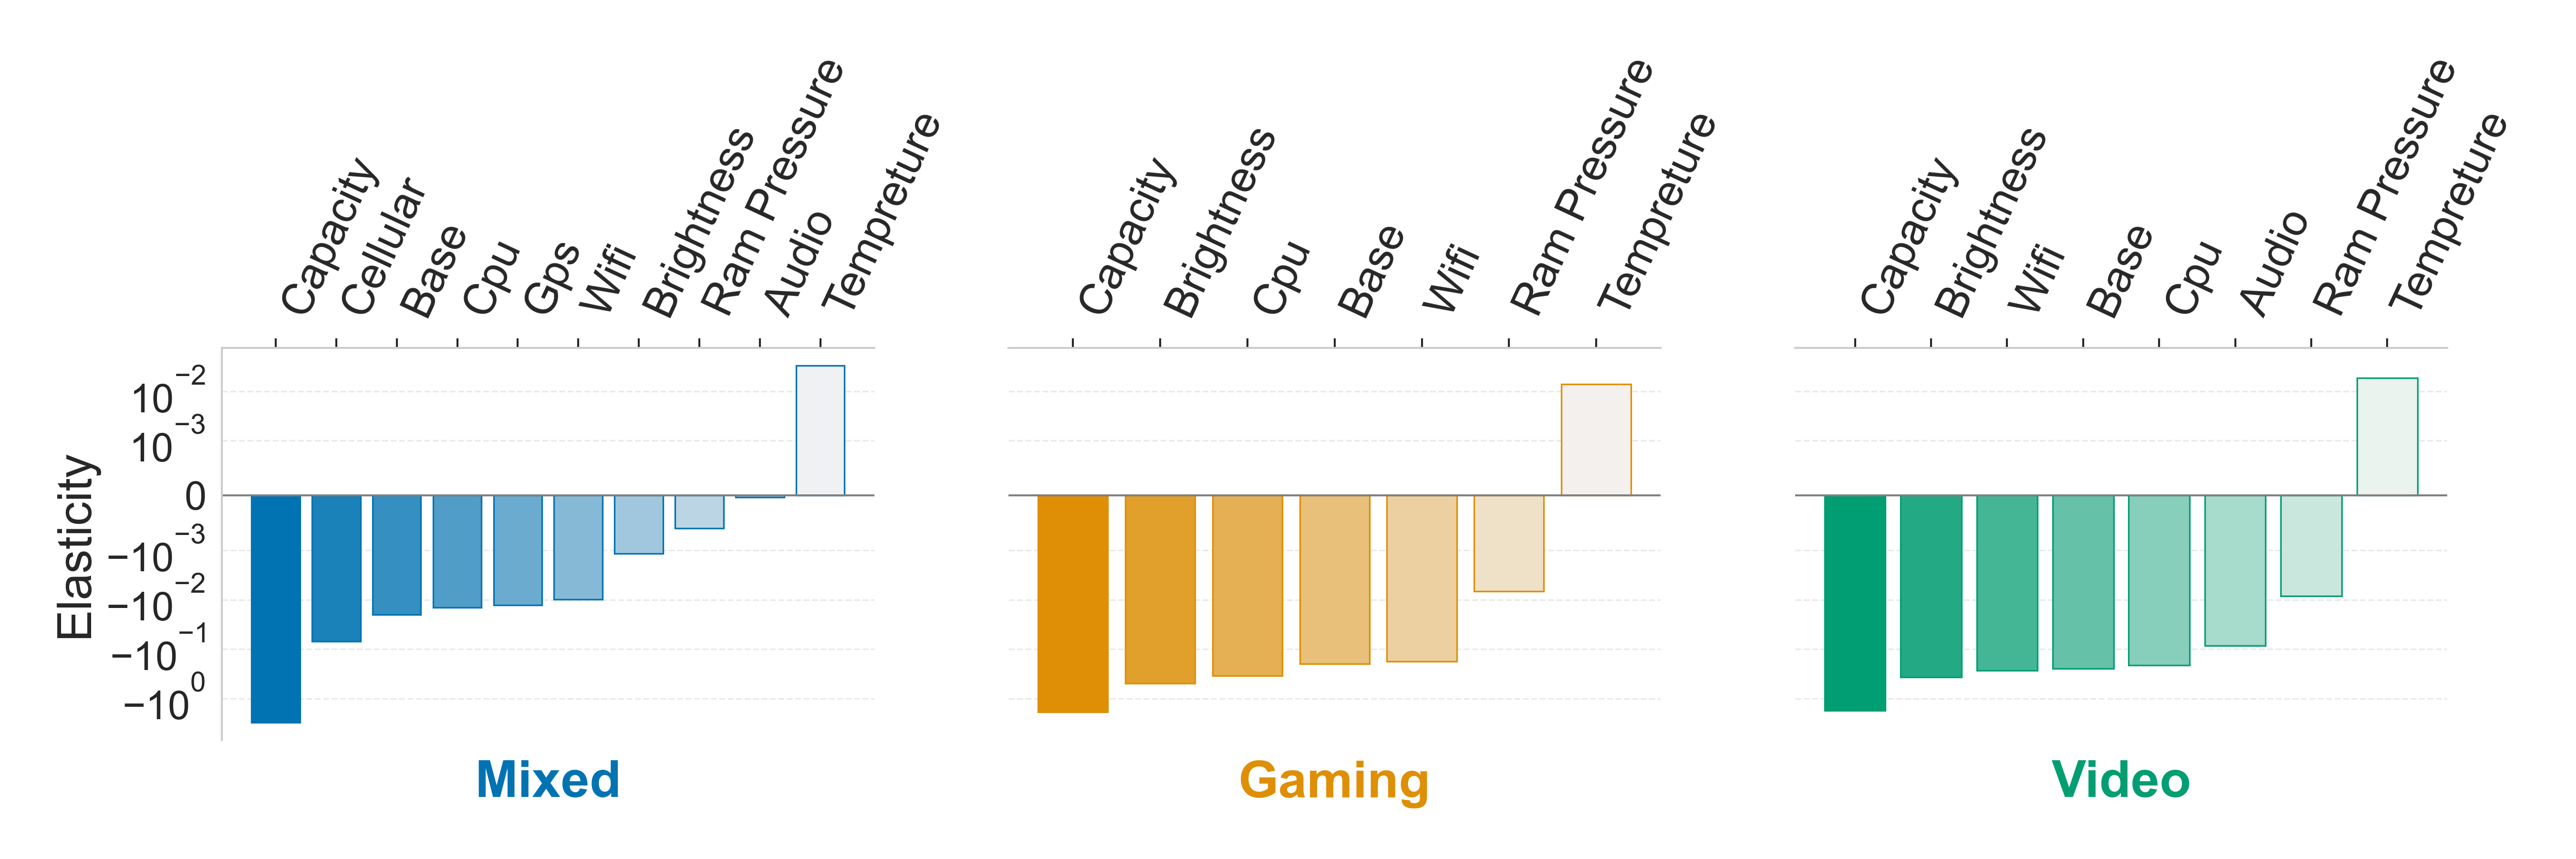
\includegraphics[width=\columnwidth]{elasticity.png}}
\caption{TTE elasticity $S_p$ across the three usage profiles.}
\label{fig:elasticity}
\end{figure}

The sensitivity results carry a practical implication for model deployment: accurate characterisation of the screen and CPU power coefficients is critical, and these should be re-fitted per device model. In contrast, GPS and audio coefficients can be reused across devices with negligible accuracy loss, reducing the per-device calibration burden.

\subsection{Component-Level Energy Attribution}

Integrating the simulated power traces by component yields the energy attribution shown in Fig.~\ref{fig:pies}. In the mixed profile, cellular and WiFi together account for roughly half the energy budget; gaming and video are CPU- and screen-heavy. The per-component breakdown enables direct diagnosis of which subsystems drive the discharge rate in a given scenario.

\begin{figure}[htbp]
\centering
\centerline{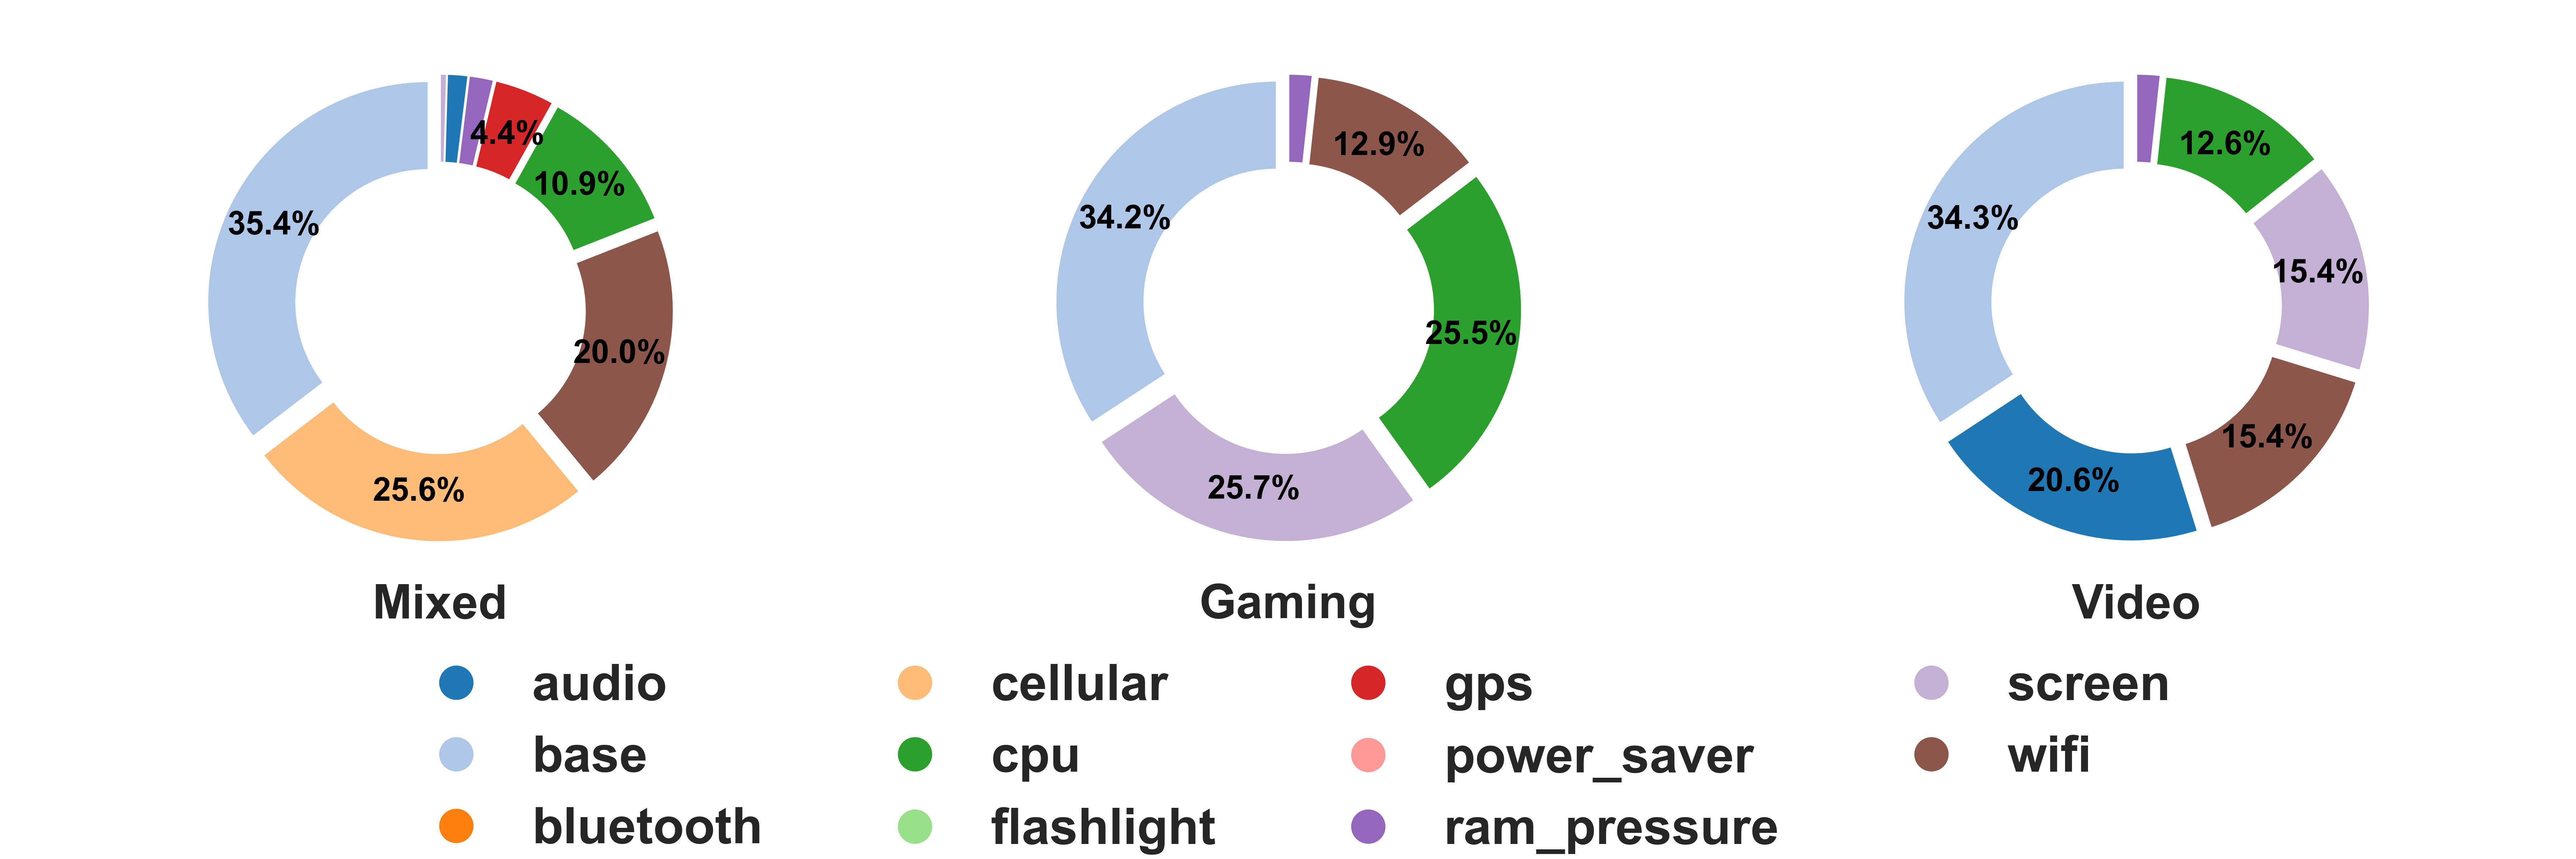
\includegraphics[width=\columnwidth]{trace_pies.png}}
\caption{Component-wise share of total energy across the three usage profiles.}
\label{fig:pies}
\end{figure}






\section{Conclusion}

In this paper, we proposed a hybrid physics-informed model for smartphone time-to-empty prediction that couples a second-order Thevenin ECM with component-level power decomposition and temperature/aging modulation. Unlike prior work that models the battery cell in isolation, the proposed framework jointly models peripheral components (screen, CPU, network radios, GPS) whose power draw dominates runtime discharge. The model parameters are fitted from authentic data collected via ADB \texttt{batterystats} on two real Android devices across three usage profiles.

Experimental results on held-out test traces demonstrate that the proposed model achieves a mean TTE MAE of \SI{0.474}{h}, outperforming the best baseline in five of six scenarios with an average reduction of \SI{16.7}{\percent}. The largest gains appear on video and mixed workloads, where the physics-informed ECM provides a structural advantage over purely statistical extrapolation. Ablation experiments confirm that both temperature correction and ECM dynamics contribute non-trivially, with their relative importance varying by workload: temperature correction is essential under wide thermal swings, while RC dynamics are most beneficial under rapidly fluctuating GPU loads. Sensitivity analysis further reveals that screen and CPU power coefficients are the dominant TTE levers and should be calibrated per device, whereas GPS and audio coefficients can be transferred across devices with negligible accuracy loss.

Future work will extend the model to capture battery aging effects from longitudinal user traces and incorporate per-user workload prediction to enable proactive power management on consumer smartphones.





\bibliographystyle{IEEEtran}
\bibliography{references}

\end{document}
